% generated by Docutils <http://docutils.sourceforge.net/>
\documentclass[a4paper,english]{article}
\usepackage{fixltx2e} % LaTeX patches, \textsubscript
\usepackage{cmap} % fix search and cut-and-paste in PDF
\usepackage{babel}
\usepackage{mathpazo}
\usepackage{setspace}
\usepackage{mathabx}
\usepackage[T1]{fontenc}
\usepackage[utf8]{inputenc}
\usepackage{ifthen}
\usepackage{float} % float configuration
\floatplacement{figure}{H} % place figures here definitely
\usepackage{graphicx}

\usepackage[colorlinks=true,linkcolor=blue,urlcolor=blue]{hyperref}
\hypersetup{
  pdftitle={Magic Lantern 0.2 for Canon 550D, Firmware 1.0.9 -- Installation},
  pdfauthor = {Alex Dumitrache <broscutamaker@gmail.com>},
  pdfpagelayout = {OneColumn},
  pdfpagemode = {UseNone},
  pdfstartview = {FitH},
  pdfborder = {0 0 0}
}
\usepackage[letterpaper, total={14.5cm, 22cm}, centering]{geometry}

\setlength{\parskip}{1.5mm plus2mm}
\setlength{\parindent}{0mm}

%%% Body
\begin{document}
\title{Magic Lantern 0.2 for Canon 550D, firmware 1.0.9\\Installation}
\author{\url{http://magiclantern.wikia.com/550D}}
\maketitle

\vspace{5mm}
\begin{center}
\setstretch{1.1}

\begin{minipage}{13cm}
\input{credits.tex}
\end{minipage}
\vspace{5mm}

\begin{minipage}{13cm}
Magic Lantern is being developed by independent film makers in our spare time and at risk to our beloved cameras. We hope that it saves you time and aggravation on set, and we'd appreciate your support. You can help by \href{https://www.paypal.com/cgi-bin/webscr?cmd=_donations&business=ELJ6U9GGFPL3U&lc=RO&item_name=Magic%20Lantern%20firmware%20for%20Canon%20550D&currency_code=EUR&bn=PP%2dDonationsBF%3abtn_donate_LG%2egif%3aNonHostedGuest}{donating via PayPal}, or through equipment donations. You can also \href{mailto:broscutamaker@gmail.com}{contact me (Alex) via email}. Thanks!

\vspace{2mm}
\hskip1mm \href{https://www.paypal.com/cgi-bin/webscr?cmd=_donations&business=ELJ6U9GGFPL3U&lc=RO&item_name=Magic%20Lantern%20firmware%20for%20Canon%20550D&currency_code=EUR&bn=PP%2dDonationsBF%3abtn_donate_LG%2egif%3aNonHostedGuest}{
\includegraphics[width=1.5cm]{donate.png}}
\end{minipage}
\end{center}


\newpage
\begin{center}
\setstretch{1.7}
\begin{minipage}{13cm}
\tableofcontents
\end{minipage}
\end{center}
\newpage



Installing Magic Lantern 0.2 for Canon 550D, Firmware 1.0.9


%___________________________________________________________________________

\section*{WARNING%
  \phantomsection%
  \addcontentsline{toc}{section}{WARNING}%
  \label{warning}%
}
%
\begin{quote}{\ttfamily \raggedright \noindent
.***************************************************\\
~*~~~~~~~~~~~~~~~~~~~~~~~~~~~~~~~~~~~~~~~~~~~~~~~~~*\\
~*~THIS~IS~DANGEROUS~AND~MIGHT~DAMAGE~YOUR~CAMERA.~*\\
~*~~NO~WARRANTIES.~~NO~GUARANTEES.~~DO~NOT~TAUNT.~~*\\
~*~~~~~~~~~~~~~~~~~~~~~~~~~~~~~~~~~~~~~~~~~~~~~~~~~*\\
~***************************************************
}
\end{quote}

If you are not comfortable with this, stop reading and delete the
software before you are tempted to try running it on your camera.

To repeat this important point:
%
\begin{quote}{\ttfamily \raggedright \noindent
.***************************************************\\
~*~~~~~~~~~~~~~~~~~~~~~~~~~~~~~~~~~~~~~~~~~~~~~~~~~*\\
~*~THIS~IS~DANGEROUS~AND~MIGHT~DAMAGE~YOUR~CAMERA.~*\\
~*~~~IF~IT~BREAKS,~YOU~GET~TO~KEEP~BOTH~PIECES.~~~~*\\
~*~~~~~~~~~~~~~~~~~~~~~~~~~~~~~~~~~~~~~~~~~~~~~~~~~*\\
~***************************************************
}
\end{quote}


%___________________________________________________________________________

\section*{Important notes%
  \phantomsection%
  \addcontentsline{toc}{section}{Important notes}%
  \label{important-notes}%
}
%
\begin{itemize}

\item EyeFi cards \href{https://bitbucket.org/hudson/magic-lantern/issue/216/eye-fi-pro-x2-doesnt-work}{are known to cause problems}, so it's better to use normal cards. See also \href{http://chdk.setepontos.com/index.php?topic=4214.msg55503\#msg55503}{this message from fe50}.

\item If you have a bootable SD card and have the \texttt{DISKBOOT} flag
set in the camera (which the installer does), and you do not have
an \texttt{AUTOEXEC.BIN} file on the card the camera \textbf{WILL NOT BOOT!}
It will hang and not wake up until the battery is removed.

\item If you encounter a ``locked up'' camera, \textbf{quickly remove the battery}.
Otherwise the ARM might be in a tight-loop and get very hot, very quickly.
Your battery will run down and your LCD might show some discoloration.

\item When in doubt, remove the battery and reboot.

\item \textbf{And, remember that this software can damage or destroy your camera.}

\end{itemize}


%___________________________________________________________________________

\section*{Introduction%
  \phantomsection%
  \addcontentsline{toc}{section}{Introduction}%
  \label{introduction}%
}

There are 2 ways of running user code on the 550D/T2i/Kiss X4:
\newcounter{listcnt0}
\begin{list}{\arabic{listcnt0}.}
{
\usecounter{listcnt0}
\setlength{\rightmargin}{\leftmargin}
}

\item using the update process with a \texttt{.fir} file, which must be digitally signed.

\item using the bootdisk process: the \texttt{autoexec.bin} file is loaded and executed.
This file does not have to be signed, but the bootdisk flag must be enabled in the camera.
\end{list}

To install Magic Lantern on your camera, you must download the right
magiclantern for your firmware: 1.0.8 or 1.0.9. The recommended way
is to upgrade your camera to 1.0.9 in order to get the latest features.

No development will be done on 1.0.8 any more.
Magic Lantern does not work at all with earlier firmware versions.


%___________________________________________________________________________

\section*{Installing Magic Lantern for 550D firmware 1.0.9 for the first time%
  \phantomsection%
  \addcontentsline{toc}{section}{Installing Magic Lantern for 550D firmware 1.0.9 for the first time}%
  \label{installing-magic-lantern-for-550d-firmware-1-0-9-for-the-first-time}%
}

\textbf{Make sure you have the Canon Firmware 1.0.9 first!}
\textbf{Running Magic Lantern on an incorrect firmware version may brick your camera!}

If you already use a previous version of Magic Lantern for 550D firmware \textbf{1.0.9}, it's easy.
Download the latest ML and unzip everything on your SD card. Done. Enjoy!

If you already use Magic Lantern for 550D/1.0.8, format your card,
upgrade camera firmware to 1.0.9 and follow the ML install steps.




%___________________________________________________________________________

\subsection*{Step 0. Downloading%
  \phantomsection%
  \addcontentsline{toc}{subsection}{Step 0. Downloading}%
  \label{step-0-downloading}%
}
%
\begin{itemize}

\item Download this release: \href{https://bitbucket.org/hudson/magic-lantern/downloads/magiclantern-0.2.0.rc1.550d.fw109.zip}{magiclantern-0.2.0.rc1.550d.fw109.zip}.

\item Read \href{http://groups.google.com/group/ml-devel/browse_thread/thread/850ec268bc883ceb}{this discussion thread} for more info.

\end{itemize}


%___________________________________________________________________________

\subsection*{Step 1. Enabling bootflag%
  \phantomsection%
  \addcontentsline{toc}{subsection}{Step 1. Enabling bootflag}%
  \label{step-1-enabling-bootflag}%
}
\begin{figure}
\noindent\makebox[\textwidth][c]{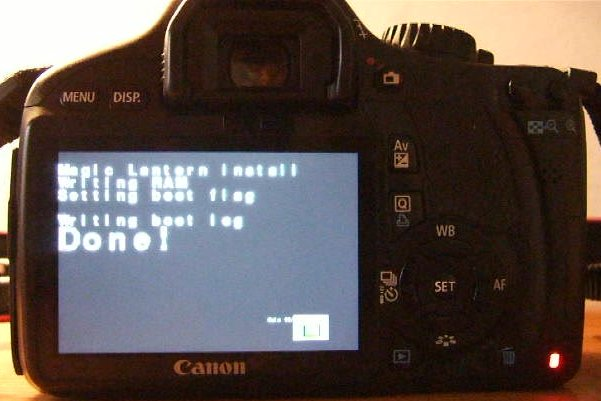
\includegraphics[width=5cm]{550install.jpg}}
\end{figure}
%
\begin{itemize}

\item Remove any accessories from your camera (such as battery grip or external flash)

\item Restore your camera to default settings (\texttt{Clear all camera settings}, from \texttt{Wrench 3} menu)

\item Format the SD card from the camera (low level, from \texttt{Wrench 1} menu)

\item Copy \texttt{magiclantern.fir} from the zip archive on the SD card

\item Launch the firmware update process. For this,
start the camera and select \texttt{Firmware ver 1.0.9} from the \texttt{Wrench 3} menu
(must be in manual or P mode to select)

\item The installer (\texttt{magiclantern.fir}) will enable the bootdisk flag in NVRAM
by calling the \texttt{bootdisk\_enable()} function from Canon firmware.

This is the \textbf{only} persistent change to your camera, which can be reverted.

\item Once the drive light has gone off and stays off for a few seconds, remove the battery.

\end{itemize}


%___________________________________________________________________________

\subsection*{Step 2. Making the SD card bootable%
  \phantomsection%
  \addcontentsline{toc}{subsection}{Step 2. Making the SD card bootable}%
  \label{step-2-making-the-sd-card-bootable}%
}

The file \texttt{autoexec.bin} can be launched if the bootdisk is enabled
AND the SD card is ``prepared'' with special values written in boot sector:
%
\begin{itemize}

\item for FAT16 cards: \texttt{EOS\_DEVELOP} at offset 43 and \texttt{BOOTDISK} at offset 64

\item for FAT32 cards: \texttt{EOS\_DEVELOP} at offset 71 and \texttt{BOOTDISK} at offset 92

\item for EXFAT cards: \texttt{EOS\_DEVELOP} at offset 130 and \texttt{BOOTDISK} at offset 122; there's also a checksum, see \href{http://magiclantern.wikia.com/wiki/Bootdisk}{Bootdisk} for details.

\end{itemize}

\textbf{Do not put an ``prepared'' (bootable) card without ``autoexec.bin`` in the camera! (it won't boot and you'll have to take the battery out).}


%___________________________________________________________________________

\subsubsection*{Mac OS X%
  \phantomsection%
  \addcontentsline{toc}{subsubsection}{Mac OS X}%
  \label{mac-os-x}%
}
\begin{figure}
\noindent\makebox[\textwidth][c]{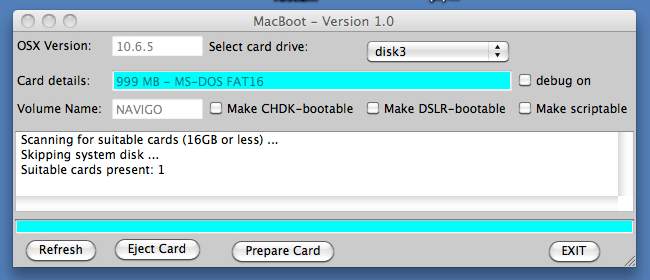
\includegraphics[width=5cm]{MacBoot.jpg}}
\end{figure}

\href{http://magiclantern.wikia.com/wiki/Video\%3AMAGIC\%20LANTERN\%201.0.9\%20HACK\%20INSTALL\%20WITH\%20A\%20MAC\%20FOR\%20CANON\%20T2I\%20OR\%20550D}{Video:MAGIC LANTERN 1.0.9 HACK INSTALL WITH A MAC FOR CANON T2I OR 550D}

Use \href{http://www.zenoshrdlu.com/macboot/macboot.html}{**MacBoot**} by \href{http://www.zenoshrdlu.com/}{Dave Mitchell}. MacBoot works with FAT16, FAT32 and EXFAT cards.

Select your SD card drive, check \texttt{Make DSLR-bootable} and hit Prepare.

If MacBoot does not work, try \texttt{make\_bootable.sh} (scroll down) and be sure to report the problem to Dave.




%___________________________________________________________________________

\subsubsection*{Windows%
  \phantomsection%
  \addcontentsline{toc}{subsubsection}{Windows}%
  \label{windows}%
}

\href{http://magiclantern.wikia.com/wiki/Video\%3AMagic\%20Lantern\%20Installation\%20Tutorial\%20for\%20Canon\%20550D\%20/\%20Rebel\%20T2i}{Video:Magic Lantern Installation Tutorial for Canon 550D / Rebel T2i}

\href{http://magiclantern.wikia.com/wiki/Video\%3ATutorial\%205\%20-\%20Magic\%20Lantern\%20by\%20Dod3032}{Video:Tutorial 5 - Magic Lantern by Dod3032}

Use \href{http://pel.hu/down/EOScard.exe}{EOScard} (thanks \href{http://pel.hu/}{Pel}!). It works with FAT16, FAT32 and EXFAT cards. You need to have Administrator rights on your Windows user account.
\begin{figure}
\noindent\makebox[\textwidth][c]{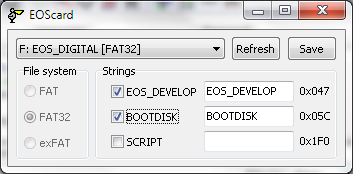
\includegraphics[width=5cm]{EOScard.png}}
\end{figure}

Select your SD card drive, check \texttt{EOS\_DEVELOP} and \texttt{BOOTDISK} and hit Save.

If the antivirus \href{https://bitbucket.org/hudson/magic-lantern/issue/207/problem-using-eoscardexe-with-bitdefender}{is complaining}, put it on Game Mode or try another operating system ;)




%___________________________________________________________________________

\subsubsection*{Linux and Mac OS X (command line)%
  \phantomsection%
  \addcontentsline{toc}{subsubsection}{Linux and Mac OS X (command line)}%
  \label{linux-and-mac-os-x-command-line}%
}

You can use \texttt{make\_bootable.sh}, which is included in the archive. If you don't know how to run scripts, see \href{http://stackoverflow.com/questions/733824/how-to-run-a-sh-script-in-an-unix-console-mac-terminal}{here}.

Open the file and change the following line in order to indicate your SD card device:
%
\begin{quote}{\ttfamily \raggedright \noindent
\#~change~this\\
dev=/dev/disk1s1
}
\end{quote}
%
\begin{itemize}

\item To find the correct \texttt{/dev/} entry under \textbf{OS X} type:
%
\begin{quote}{\ttfamily \raggedright \noindent
diskutil~list~|~grep~FAT
}
\end{quote}

That will list all mounted FAT disks, the \texttt{/dev/} entry is the last column. Note also that under OS X this script will leave the card unmounted, eject and reinsert it to re-mount it.

\item To find the correct \texttt{/dev/} entry under \textbf{Linux} type:
%
\begin{quote}{\ttfamily \raggedright \noindent
mount~|~grep~fat
}
\end{quote}

and choose the one labeled \texttt{EOS\_DIGITAL}.

\item For EXFAT cards, see \href{http://groups.google.com/group/ml-devel/browse_thread/thread/1dae47529094cae3}{this thread}.

\end{itemize}

Run the script from the terminal:
%
\begin{quote}{\ttfamily \raggedright \noindent
bash~make\_bootable.sh
}
\end{quote}

If it doesn't have enough permissions, run it as root:
%
\begin{quote}

sudo bash make\_bootable.sh

\end{quote}


%___________________________________________________________________________

\subsection*{Step 3. The last one :)%
  \phantomsection%
  \addcontentsline{toc}{subsection}{Step 3. The last one :)}%
  \label{step-3-the-last-one}%
}
%
\begin{itemize}

\item Delete \texttt{magiclantern.fir}.

\item Copy \texttt{autoexec.bin} and \texttt{cropmks} on your SDCard. Older builds may require some BMP files and \texttt{magic.cfg}.

\item Put the card in the camera.

\item Switch on your camera, and Magic Lantern (\texttt{autoexec.bin}) will boot.

\end{itemize}

As long as you had enabled the \texttt{BOOTDISK} flag once, you card is ``prepared'';
the camera will try to load any \texttt{autoexec.bin}. The \texttt{.fir} file is not needed any more,
unless for some reason you will want to retry the installation process.


%___________________________________________________________________________

\subsection*{Troubleshooting%
  \phantomsection%
  \addcontentsline{toc}{subsection}{Troubleshooting}%
  \label{troubleshooting}%
}
%
\begin{itemize}

\item Check if all doors are closed. The camera will not boot if the SD slot door is open!

\item If Magic Lantern does not work (i.e. no new features are noticed), repeat Step 2. This means your card is not bootable. Also try with an older (FAT16) card, try with another card reader, another PC or another operating system.

\item \textbf{DO NOT repeat the firmware upgrade step with ``magiclantern.fir``}! There may be a firmware update counter like on the 7D, and you may end up with a bricked camera.

\item If the camera does not boot (seems dead), \textbf{remove the battery and the card}.
Then put the battery back and try to boot the camera without card. Then put a formatted card
in the camera and try to boot \textbf{without} Magic Lantern. Only after you are sure the camera is OK,
you can try to see what's wrong with Magic Lantern.

\item \textbf{Again, NEVER let a prepared card without a working autoexec.bin on it, remove the battery immediatly during 5 seconds, switching off is not enough !!!}

\item Look in the \href{https://bitbucket.org/hudson/magic-lantern/issues}{issue tracker} for similar problems; if you can't find the solution, create a new issue there.

\end{itemize}


%___________________________________________________________________________

\section*{Installing updated Magic Lantern builds%
  \phantomsection%
  \addcontentsline{toc}{section}{Installing updated Magic Lantern builds}%
  \label{installing-updated-magic-lantern-builds}%
}

\href{http://magiclantern.wikia.com/wiki/Video\%3A550D\%20T2I\%20Magic\%20Lantern\%3A\%20Installing\%20New\%20Builds\%2C\%20Offical\%20/\%20ML\%20in\%20parallel\%2C\%20Deinstalling\%20ML}{Video:550D T2I Magic Lantern: Installing New Builds, Offical / ML in parallel, Deinstalling ML}

\href{http://magiclantern.wikia.com/wiki/Video\%3AMAGIC\%20LANTERN\%201.0.9\%20FIRMWARE\%20HACK\%3AUPDATE\%20Q\%26A}{Video:MAGIC LANTERN 1.0.9 FIRMWARE HACK:UPDATE Q\&A}

After you've installed ML, you can get updated builds; just unzip them on the SD card (overwrite old files).

It's highly recommended to install an updated build, usually the last one. They are announced first on the \href{http://groups.google.com/group/ml-devel}{ML mailing list} and on \href{http://vimeo.com/groups/magiclantern/forumthread:236203}{Vimeo Magic Lantern User Group}.

Make sure you have the correct firmware version!




%___________________________________________________________________________

\section*{Uninstalling Magic Lantern%
  \phantomsection%
  \addcontentsline{toc}{section}{Uninstalling Magic Lantern}%
  \label{uninstalling-magic-lantern}%
}


%___________________________________________________________________________

\subsection*{Uninstalling ML from one card%
  \phantomsection%
  \addcontentsline{toc}{subsection}{Uninstalling ML from one card}%
  \label{uninstalling-ml-from-one-card}%
}

Format the card from the camera, and Magic Lantern will be gone (only from that card, of course).

\textbf{Don't} just delete the Magic Lantern files from the card! If you do, the camera won't boot and you'll have to take the battery out.


%___________________________________________________________________________

\subsection*{Uninstalling ML from the camera%
  \phantomsection%
  \addcontentsline{toc}{subsection}{Uninstalling ML from the camera}%
  \label{uninstalling-ml-from-the-camera}%
}

\textbf{You don't have to do this} unless you are asked to do so by ML developers. For most users, formatting the card will be enough to uninstall ML.

If you know what you are doing, put this in \texttt{magic.cfg} to reset the \texttt{DISKBOOT} flag from the camera:
%
\begin{quote}{\ttfamily \raggedright \noindent
magic.disable\_bootdiskf~=~1
}
\end{quote}


%___________________________________________________________________________

\section*{Older versions (archived)%
  \phantomsection%
  \addcontentsline{toc}{section}{Older versions (archived)}%
  \label{older-versions-archived}%
}


%___________________________________________________________________________

\subsection*{550D/1.0.9%
  \phantomsection%
  \addcontentsline{toc}{subsection}{550D/1.0.9}%
  \label{d-1-0-9}%
}
%
\begin{itemize}

\item 3 Dec 2010: \href{http://bitbucket.org/hudson/magic-lantern/downloads/magiclantern-0.1.9-rc0_550d_fw109.zip}{magiclantern-0.1.9-rc0\_550d\_fw109.zip}

\end{itemize}


%___________________________________________________________________________

\subsection*{550D/1.0.8%
  \phantomsection%
  \addcontentsline{toc}{subsection}{550D/1.0.8}%
  \label{d-1-0-8}%
}

No further development will be done on the 1.0.8 firmware.


%___________________________________________________________________________

\subsubsection*{Official builds from Trammell Hudson%
  \phantomsection%
  \addcontentsline{toc}{subsubsection}{Official builds from Trammell Hudson}%
  \label{official-builds-from-trammell-hudson}%
}
%
\begin{itemize}

\item \href{http://groups.google.com/group/ml-devel/msg/49631dc8fec89779}{Announcing pre-alpha firmware}

\item RC1 release: \href{http://bitbucket.org/hudson/magic-lantern/downloads/magiclantern-550d.rc1.zip}{magiclantern-550d.rc1.zip}

\item 8 Aug 2010: \href{http://groups.google.com/group/ml-devel/browse_thread/thread/1192bdeeb58e94d5}{Update 550D beta, now with gain control}

\end{itemize}


%___________________________________________________________________________

\subsubsection*{Unofficial (experimental) builds%
  \phantomsection%
  \addcontentsline{toc}{subsubsection}{Unofficial (experimental) builds}%
  \label{unofficial-experimental-builds}%
}
%
\begin{itemize}

\item 11 Nov 2010: \href{http://groups.google.com/group/ml-devel/msg/87b96d3cb43b4bec}{magiclantern for 550D, compiled with shorter config file}

\item 23 Nov 2010: \href{http://groups.google.com/group/ml-devel/msg/1c690d8dee580ee3}{Recording Internal and external audio simultaneously}

\item 07 Dec 2010: \href{http://groups.google.com/group/ml-devel/msg/5abd238291b1d2b3}{fixed cropmarks}

\item 09 Dec 2010: \href{http://groups.google.com/group/ml-devel/browse_thread/thread/e15fac669f293d2a}{enabled zebras and histogram}

\item 11 Dec 2010: \href{http://groups.google.com/group/ml-devel/browse_thread/thread/97488a67eff87b7e}{GUI menus \& lots of extras}

\item 12 Dec 2010: \href{http://groups.google.com/group/ml-devel/msg/0dbfe7d9ee043525}{enabled QScale and spotmeter}

\end{itemize}


%___________________________________________________________________________

\section*{Risks%
  \phantomsection%
  \addcontentsline{toc}{section}{Risks}%
  \label{risks}%
}
%
\begin{itemize}

\item This firmware does a (very small) (semi-)permanent change to your camera: it changes the \texttt{DISKBOOT} flag, which is stored in NVRAM. This change can be reverted (see the mailing list and bootflags.c).

\item There are no confirmed reports of Magic Lantern doing permanent damage on the 550D.

However, there are reports on CHDK forum that some users \href{http://chdk.setepontos.com/index.php?topic=4202.315}{bricked their 350D}, most probably by installing a hack on the wrong firmware version. There are also lots of reports of camera refusing to boot after installing ML; this happens because they have tried to start the camera from a bootable (i.e. prepared) card without \texttt{autoexec.bin}.

\item Starting the camera with a bootable card without an \texttt{autoexec.bin} \textbf{will cause symptoms similar to a bricked one} (it will not boot). This may scare you. If it happens, \textbf{take the battery out quickly} and the camera should be fine. There are many reports about cameras which behave like being bricked, when in fact it was just \texttt{autoexec.bin} missing. That's why you should read the install instructions carefully.

\item On certain cameras, there are power management issues (i.e. if you turn off the camera or let it go to standby, it won't start any more). Make sure you don't have these problems; if you do, take the battery out after each shooting session!

\item Even if you don't have power issues, it's a good idea to take the battery out when you don't use the camera.

\item The biggest risk is when experimenting with source code without knowing what you are doing. Calling certain functions or calling them at the wrong moment can be dangerous.

\item Risks are low with pre-built binaries, since we test them on our cameras before making them public.

\item Risks are minimal with official versions (from the main repo), since they get tested by many users before releasing them.

\end{itemize}

That being said, Magic Lantern for 550D was downloaded over 10000 times (without counting downloads from the mailing list or from other sites), and most users run it successfully and use it for production, not only for testing.


%___________________________________________________________________________

\section*{Source code%
  \phantomsection%
  \addcontentsline{toc}{section}{Source code}%
  \label{source-code}%
}

You can build your own \texttt{AUTOEXEC.BIN} files with \href{http://bitbucket.org/hudson/magic-lantern/overview}{the 550d branch of the
source code}:
%
\begin{quote}{\ttfamily \raggedright \noindent
hg~clone~-r~550d~https://bitbucket.org/hudson/magic-lantern
}
\end{quote}

There is \textbf{no} Canon source or object code in the Magic Lantern tree
and we do \textbf{not} distribute ROM dumps since they contain code that is
copyright by Canon. If you have the camera in hand, you can make your own
dump for analysis and use \href{http://groups.google.com/group/ml-devel/browse_thread/thread/e134ff54ae181c36}{this IDC database}
to add symbols to it.

If you want to compile your own \texttt{AUTOEXEC.BIN}, check the following wiki pages:
%
\begin{itemize}

\item \href{http://magiclantern.wikia.com/wiki/For\%20Developers}{For Developers}

\item \href{http://magiclantern.wikia.com/wiki/Build\%20instructions/550D}{Build instructions/550D}

\item \href{http://magiclantern.wikia.com/wiki/550d\%20dev}{550d dev}

\end{itemize}

\end{document}


